\chapter[Appendix 3]{Appendix 3 (supplementary to Chapters 2 and 3)}

\section{Study regions in Chapters 2-4}

%%%% FIGURE 1
\begin{figure}[ht]
\begin{center}
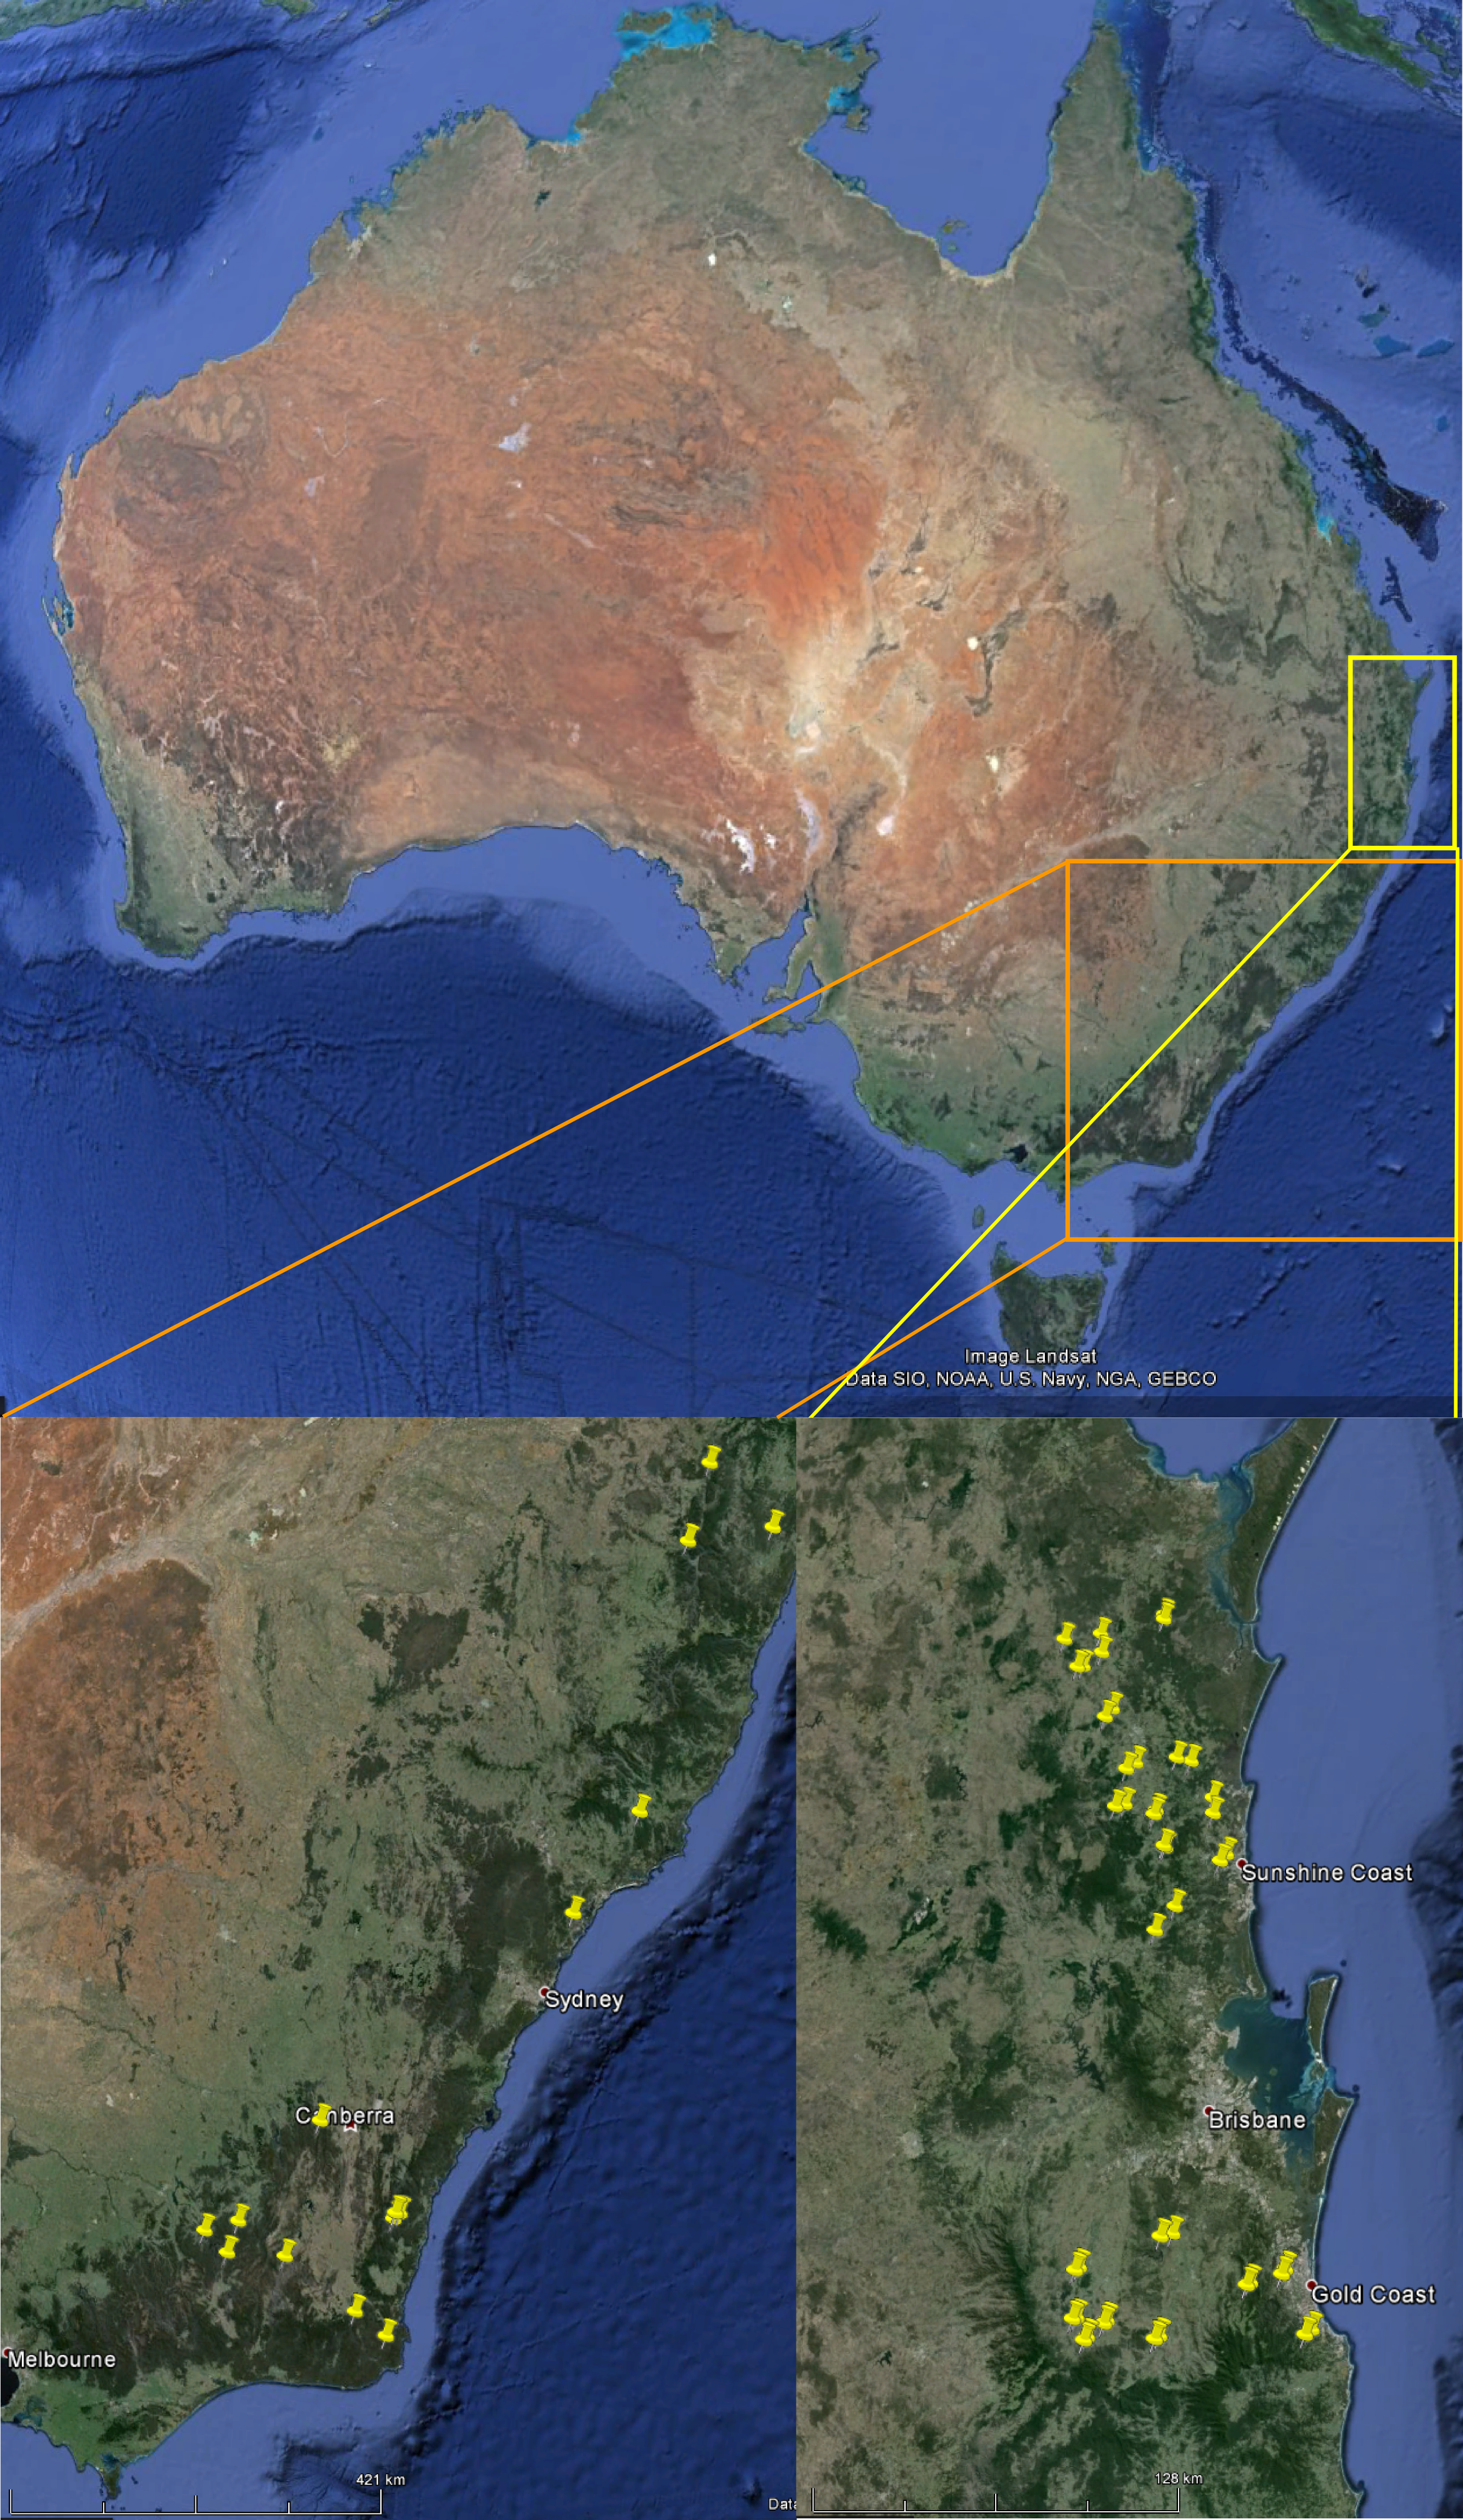
\includegraphics[width=12cm,keepaspectratio=true]{Ch6map.png} % figures can be in pdf, png, jpeg or eps format
\caption[Map of study areas described in Chapters 2-4.]{\small{Map showing study areas, and geographical distribution of field sites described in Chapters 2 \& 3 (lower left) and 4 (lower right) (Google Maps 2015).}\label{fig:Ch6_F1}}
%\label{Ch6_F1} % label for cross-referencing
\end{center}
\end{figure}   
\clearpage

\section{Biophysical characteristics of study sites}

This section describes the biophysical characteristics of study sites used in Chapters 2 and 3. For further information about study sites used in Chapter 4, the reader is referred to \citep{Arthington2012}.

\subsection{Biogeography}


\begin{table}[]
\centering
\caption{My caption}
\label{my-label}
\begin{tabular}{lllllll}
Site                                   & IBRA region              & Koppen climate zone           & Mean annual rainfall (mm) & Mean annual temperature (oC) & Upstream catchment area (m2) & elevation (m asl) \\
Mammy Johnsons River at Pikes Crossing & NSW North Coast          & Warm summer, cold winter      & 1136                      & 17.5                         & 158                          & 104               \\
Wallagaraugh River at Princes Highway  & South East Corner        & Warm summer, cold winter      & 925                       & 14.9                         & 477                          & 35                \\
Genoa River at Bondi                   & South East Corner        & Warm summer, cold winter      & 815                       & 13.0                         & 234                          & 417               \\
Wadbilliga River at Wadbilliga         & South East Corner        & Warm summer, cold winter      & 842                       & 14.8                         & 126                          & 201               \\
Tuross River D/S Wadbilliga Junction   & South East Corner        & Warm summer, cold winter      & 843                       & 15.4                         & 918                          & 79                \\
Tuross River at Belowra                & South East Corner        & Warm summer, cold winter      & 831                       & 15.4                         & 564                          & 105               \\
Jacobs River at Jacobs Ladder          & South Eastern Highlands  & Mild-warm summer, cold winder & 563                       & 13.9                         & 184                          & 343               \\
Nariel Creek at Upper Nariel           & South Eastern Highlands  & Mild-warm summer, cold winder & 982                       & 12.8                         & 261                          & 711               \\
Gibbo River at Gibbo Park              & South Eastern Highlands  & Mild-warm summer, cold winder & 919                       & 12.5                         & 390                          & 515               \\
Snowy Creek at Below Granite Flat      & South Eastern Highlands  & Mild-warm summer, cold winder & 1030                      & 13.8                         & 416                          & 331               \\
Mann River at Mitchell                 & New England Tablelands   & Warm summer, cold winter      & 865                       & 16.7                         & 890                          & 401               \\
Cataract Creek at Sandy Hill           & New England Tablelands   & Warm summer, cold winter      & 1019                      & 16.4                         & 237                          & 595               \\
Sportsmans Creek at Gurranang Siding   & South Eastern Queensland & Warm humid summer             & 1094                      & 19.1                         & 205                          & 13                \\
Goodradigbee River at Brindabella      & South Eastern Highlands  & Mild-warm summer, cold winder & 976                       & 12.7                         & 432                          & 510               \\
Jilliby Creek at U/S Wyong River       & Sydney Basin             & Warm summer, cold winter      & 1110                      & 17.7                         & 93                           & 39               
\end{tabular}
\end{table}


\subsection{Fluvial geomorphology}

-	Valley extent and confinement
-	Substrate
-	Field sampling design?


\subsection{Vegetation and site history}



\begin{table}[]
\centering
\caption{My caption}
\label{my-label}
\begin{tabular}{lllll}
Site                                   & Canopy height (m) & Vegetation structure                                                    & Dominant species                                                                                                                          & Site history                                                                                                                                                                                           \\
Mammy Johnsons River at Pikes Crossing & 15                & Closed canopy, abundant subcanopy and limited groundcover               & Acmena smithii, Ceratopetalum apetalum, Tristaniopsis laurina                                                                             & Adjacent smallhold grazing, unfenced, possible historic clearing                                                                                                                                       \\
Wallagaraugh River at Princes Highway  & 12                & Closed low canopy, fern dominated groundcover layer                     & Tristaniopsis laurina, Doodia aspera                                                                                                      & Undisturbed, evidenced by numerous large Eucalyptus viminalis individuals adjacent to site                                                                                                             \\
Genoa River at Bondi                   & 30                & Tall open canopy, abundant subcanopy and groundcover                    & Eucalyptus viminalis, Pomaderris aspera, Leptospermum brevipes, Calochlaena dubia                                                         & Undisturbed, within South East Forest National Park                                                                                                                                                    \\
Wadbilliga River at Wadbilliga         & 30                & Tall open canopy, abundant shrubs and groundcover                       & Casuarina cunninghamiana, Eucalyptus cypellocarpa, Acacia floribunda, Melicytus dentatus, Microlaena stipoides                            & Within Wadbilliga National Park. Mature forest, but historical clearing / pastoral land use possible.                                                                                                  \\
Tuross River D/S Wadbilliga Junction   & 30                & Open forest, shrub and groundcover layers dominant, scattered emergents & Casuarina cunninghamiana, Eucalyptus elata, Tristaniopsis laurina, Acacia floribunda, Backhousia myrtifolia, Microlaena stipoides         & Within Wadbilliga National Park. Mature forest with large emergents, but historical clearing / pastoral land usepossible.                                                                              \\
Tuross River at Belowra                & 12                & Riparian scrub with emergent streamside Casuarina forest                & Casuarina cunninghamiana, Acacia floribunda, Leptospermum brevipes                                                                        & Within Wadbilliga National Park. Mature riparian scrub vegetation, but historical clearing / pastoral land use possible.                                                                               \\
Jacobs River at Jacobs Ladder          & 14                & Open woodland with some emergent Eucalypts                              & Eucalyptus rubida, Acacia dealbata, Rubus fruticosus                                                                                      & Within Kosciuzko National Park. In recovery following 2003 fires.                                                                                                                                      \\
Nariel Creek at Upper Nariel           & 40                & Open forest, dense fern groundcover                                     & Eucalyptus camphora subsp. humeana, Acacia melanoxylon, Rubus fruticosus, Blechnum nudum                                                  & Mature forest, some clearing adjacent to riparian corridor. Historical clearing / pastoral land use possible.                                                                                          \\
Gibbo River at Gibbo Park              & 35                & Open forest, abundant shrub layer                                       & Eucalyptus radiata, Acacia dealbata, Lomatia myricoides, Poa labillardierei var labillardierei                                            & Largely undisturbed, some evidence of fire. Within Alpine National Park. Very large emergent Eucalyptus viminalis (>2m DBH) present.                                                                                       \\
Snowy Creek at Below Granite Flat      & 20                & Riparian scrub with low emergent Eucalypts                              & Eucalyptus camphora subsp. camphora, Eucalyptus stellulata, Coprosma quadrifida, Bursaria spinosa, Leptospermum brevipes                  & Within Victoria State Forest, clearing for forestry was evident downstream.                                                                                                                            \\
Mann River at Mitchell                 & 30                & Open grassy forest                                                      & Casuarina cunninghamiana, Eucalyptus ampifolia, Lomandra longifolia, Microlaena stipoides                                                 & Within Mann River Nature Reserve. Large flood occurred in 2011, historical clearing / pastoral land use is possible.                                                                                   \\
Cataract Creek at Sandy Hill           & 30                & Open forest, abundant shrubs and grassy areas                           & Casuarina cunninghamiana, Eucalyptus tereticornis, Melicytus dentatus, Lomandra hystrix, Pennisetum clandestinum                          & Within NSW conservation land, although opposite side of river was cleared pastoral land. Large flood occurred in 2011.                                                                                 \\
Sportsmans Creek at Gurranang Siding   & 25                & Closed forest                                                           & Lophostemon suaveolens, Alphitonia excelsa, Casuarina glauca, Calochlaena dubia, Oplismenus imbecillis                                    & Riparian corridor remnant vegetation. Adjacent to Gunnarang State Conservation Area. Large (\textgreater2m DBH) emergent Lophostemon suaveolens individuals indicate relatively undisturbed condition. \\
Goodradigbee River at Brindabella      & 25                & Closed forest, abundant shrub layer with sparse groundcover             & Eucalyptus radiata, Eucalyptus viminalis, Acacia dealbata, Acacia pravissima, Hovea asperifolia subsp. asperifolia, Leptospermum brevipes & Within Kosciuzko National Park. Fire occurred in 2010.                                                                                                                                                 \\
Jilliby Creek at U/S Wyong River       & 50                & Vine thickets with emergent Eucalypts                                   & Eucalyptus tereticornis, Eucalyptus resinifera, Commersonia fraseri, Ripogonum album, Lomandra longifolia                                 & Riparian corridor remnant vegetation. Large emergent Eucalyptus individuals (40-50 m tall) indicate relatively undisturbed condition.                                                                 
\end{tabular}
\end{table}




PHOTOS









